\documentclass[tikz,border=4pt]{standalone}
% Estilo común de los diagramas de bloques (se usa con \input en cada standalone)
\usepackage[defaultsans,scale=0.92]{lato}
\usepackage{libertinust1math}
\usepackage{xcolor,amsmath}
\usepackage{tikz}
\usetikzlibrary{positioning,arrows.meta,calc,shapes.geometric}
\usepackage{../../notacion}
\definecolor{ctrlazul}{HTML}{1E5AA8}\definecolor{ctrlnoche}{HTML}{14213D}
\definecolor{ctrlcoral}{HTML}{D1495B}\definecolor{ctrlverde}{HTML}{2A9D8F}
\definecolor{ctrlambar}{HTML}{E09F3E}\definecolor{ctrlgris}{HTML}{5C677D}
\definecolor{ctrlvioleta}{HTML}{6C4AB6}\definecolor{ctrlteal}{HTML}{0F7173}
\tikzset{
  >={Stealth[length=2.4mm]}, every node/.style={font=\small},
  bloque/.style={draw=ctrlnoche,fill=ctrlazul!7,thick,rounded corners=1.5pt,minimum height=9mm,minimum width=13mm,inner sep=4pt},
  suma/.style={draw=ctrlnoche,thick,circle,inner sep=0pt,minimum size=6mm},
  senal/.style={->,thick,draw=ctrlnoche},
  rot/.style={font=\footnotesize,text=ctrlgris},
}

\usetikzlibrary{decorations.pathmorphing,patterns}
\begin{document}
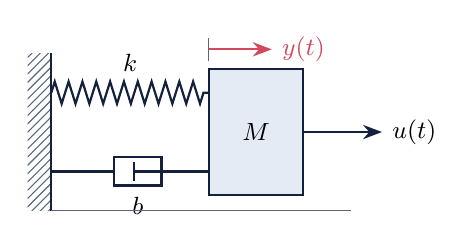
\begin{tikzpicture}[font=\small]
  \fill[pattern=north east lines,pattern color=ctrlgris] (-0.3,-0.2) rectangle (0,1.8);
  \draw[thick,ctrlnoche] (0,-0.2)--(0,1.8);
  \draw[thick,ctrlnoche,decorate,decoration={zigzag,segment length=5pt,amplitude=4pt}] (0,1.3)--(2,1.3);
  \node[above] at (1,1.45) {$k$};
  \draw[thick,ctrlnoche] (0,0.3)--(0.8,0.3); \draw[thick,ctrlnoche] (0.8,0.12) rectangle (1.4,0.48);
  \draw[thick,ctrlnoche] (1.05,0.3)--(2,0.3); \draw[thick,ctrlnoche] (1.05,0.18)--(1.05,0.42);
  \node[below] at (1.1,0.1) {$b$};
  \draw[thick,ctrlnoche,fill=ctrlazul!12] (2,0) rectangle (3.2,1.6); \node at (2.6,0.8) {$M$};
  \draw[senal] (3.2,0.8)--(4.2,0.8) node[right]{$u(t)$};
  \draw[->,thick,ctrlcoral] (2,1.85)--(2.8,1.85) node[right]{$y(t)$};
  \draw[ctrlgris] (2,1.7)--(2,2.0);
  \draw[ctrlgris] (0,-0.2)--(3.8,-0.2);
\end{tikzpicture}
\end{document}
